\documentclass[a4paper,12pt]{article}
\usepackage[utf8]{inputenc}
\usepackage{geometry}
\usepackage{longtable}
\usepackage{booktabs}
\usepackage{enumitem}
\usepackage{xcolor}
\usepackage{caption}
\usepackage{graphicx}

\geometry{margin=1in}

\title{\textbf{Personal Investment Report for 2025 Q1}}
\author{Yi-Fan Chen}
\date{April 7, 2025}

\begin{document}

\begin{titlepage}
    \centering
    \vspace*{\fill}
    {\Huge \textbf{PIGU INVESTMENT, INC.} \par}
    \vspace{1.5cm}
    {\LARGE Balance Sheet \par}
    \vspace{2cm}
    {\Large April 2025 Quarter 1 \par}
    \vspace*{\fill}
\end{titlepage}


\section{Introduction}
This report provides an overview of my investment portfolio as of April 2025, including current holdings, realized and unrealized gains/losses, and cash reserves.

\section{Current Holdings (NTD)}
\begin{longtable}{llllll}
    \toprule
    Stock Code & Shares & Avg. Purchase Price & Current Market Price & Cost & Value \\
    \midrule
    2884 E.SUN F      & 1020 & 24.26 & 26.6  & 24,745.2 & 27,081 \\
    2912 PCSC         & 150  & 254.35 & 243.5 & 38,152.5 & 36,450 \\
    2916 Munsin       & 750  & 49.93 & 47.55 & 37,447.5 & 35,663 \\
    2379 Realtek      & 60   & 487.32 & 442.0 & 29,239.2 & 26,490 \\
    2610 China Air    & 500  & 19.3   & 19.6  & 9,650   & 9,800 \\
    \bottomrule
\end{longtable}

\section{Realized Gains/Losses (NTD)}
\begin{longtable}{lllll}
    \toprule
    Stock Code & Shares & Buy Price & Sell Price & Gain/Loss \\
    \midrule
    00940 Yuanta High Dividend ETF & 1000 & 9.85 & 7.9  & -1,917 \\
    1301 Formosa Plastics          & 200  & 50.3 & 34.8 & -3,143 \\
    \bottomrule
\end{longtable}
\textbf{Total Realized Loss:} \textcolor{red}{-5,060} NTD

\section{Unrealized Gains/Losses}
\begin{longtable}{ll}
    \toprule
    Stock Code & Gain/Loss (NTD) \\
    \midrule
    E.SUN Financial       & 2,284 \\
    President Chain Store & -1,938 \\
    Munsin Garment        & -1,943 \\
    Realtek               & -2,925 \\
    China Airlines        & 150 \\
    \bottomrule
    \textbf{Total Unrealized Loss:} & \textcolor{red}{-4,372} \\
\end{longtable}

\section{Stock Equity Distribution}
\begin{figure}[h!]
    \centering
    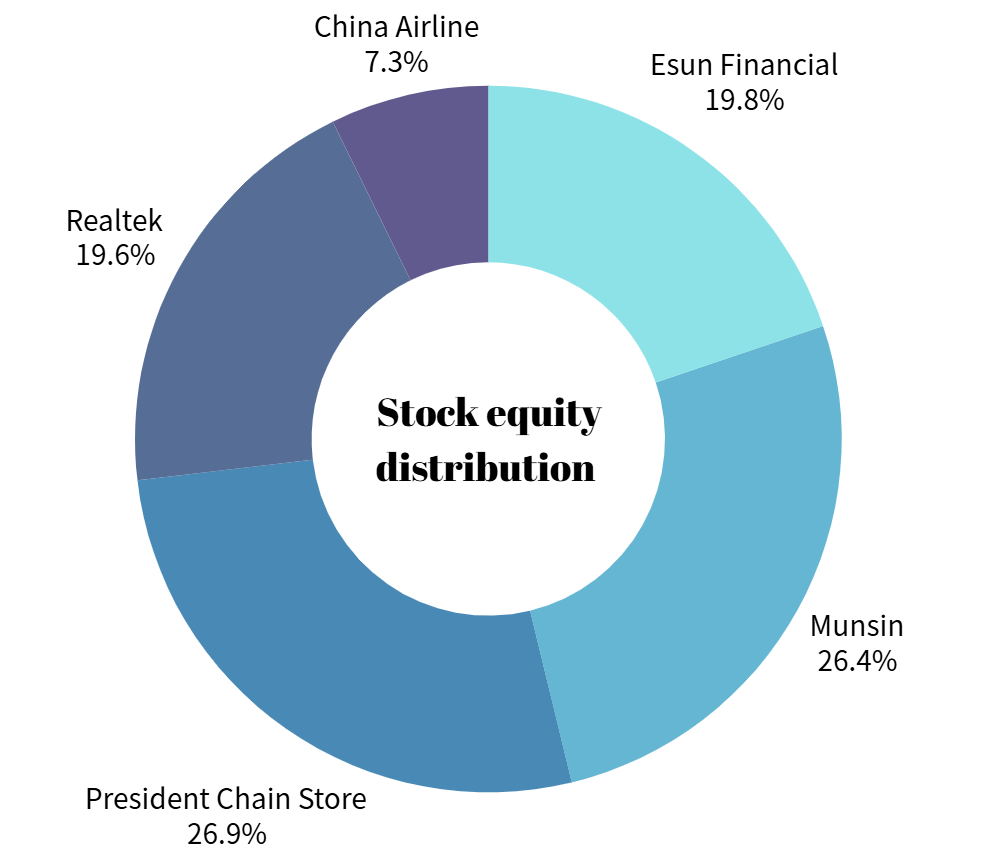
\includegraphics[width=0.8\textwidth]{stock_equity_distribution.png}
    \caption{Stock Equity Distribution as of 2025 Q1}
    \label{fig:stock_equity_distribution}
\end{figure}

\noindent The figure below illustrates the distribution of stock equity in my portfolio as of the first quarter of 2025. It provides a visual representation of the proportion of each stock's value relative to the total portfolio value.

\section{Total Profit/Loss Summary}
\begin{longtable}{ll}
    \toprule
    Category & Amount (NTD) \\
    \midrule
    Realized   & -5,060 \\
    Unrealized & -4,372 \\
    \midrule
    \textbf{Overall Total} & \textcolor{red}{-9,432} \\
    \bottomrule
\end{longtable}

\section{Cash \& Fixed Deposits}
\begin{longtable}{ll}
    \toprule
    Type & Amount (NTD) \\
    \midrule
    USD Fixed Deposit (9,628 USD @ 32.9) & 316,761 \\
    TWD Cash                             & 30,000 \\
    \bottomrule
    \textbf{Total Cash} & 346,761 \\
\end{longtable}

\noindent
The large proportion of USD fixed deposits is due to the current high interest rate of 2.5\%. To achieve better asset allocation and reduce risk, it was decided not to adjust the USD fixed deposit.

\section{Total Equity}
\begin{longtable}{ll}
    \toprule
    Category & Amount (NTD) \\
    \midrule
    Total Portfolio Value (Holdings) & 135,165 \\
    Total Cash \& Deposit            & 346,761 \\
    \bottomrule
    \textbf{Total Equity} & 481,956 \\
\end{longtable}

\end{document}
